\section{Ilham Muhammad Ariq (1174087)}
\subsection{Menulis Shapefile dengan PySHP}
\begin{enumerate}
	\item Nomor 1
	\lstinputlisting{src/tugas2/1174087/no1.py}
	\begin{figure}[H]
		
\includegraphics[width=6cm]{figures/Tugas2/1174087/no1.jpg}
		\centering
		\caption{Point (Titik)}
	\end{figure}
	\item Nomor 2
	\lstinputlisting{src/tugas2/1174087/no2.py}
	\begin{figure}[H]
		
\includegraphics[width=6cm]{figures/Tugas2/1174087/no2.jpg}
		\centering
		\caption{Point (Titik)}
	\end{figure}
	\item Nomor 3
	\lstinputlisting{src/tugas2/1174087/no3.py}
	\begin{figure}[H]
		
\includegraphics[width=6cm]{figures/Tugas2/1174087/no3.jpg}
		\centering
		\caption{Point (Titik)}
	\end{figure}
	\item Nomor 4
	\lstinputlisting{src/tugas2/1174087/no4.py}
	\begin{figure}[H]
		
\includegraphics[width=6cm]{figures/Tugas2/1174087/no4.jpg}
		\centering
		\caption{Point (Titik)}
	\end{figure}
	\item Nomor 5
	\lstinputlisting{src/tugas2/1174087/no5.py}
	\begin{figure}[H]
		
\includegraphics[width=6cm]{figures/Tugas2/1174087/no5.jpg}
		\centering
		\caption{PolyLine (Garis)}
	\end{figure}
	\item Nomor 6
	\lstinputlisting{src/tugas2/1174087/no6.py}
	\begin{figure}[H]
		
\includegraphics[width=6cm]{figures/Tugas2/1174087/no6.jpg}
		\centering
		\caption{Polygon (Bidang)}
	\end{figure}
	\item Nomor 7
	\lstinputlisting{src/tugas2/1174087/no7.py}
	\begin{figure}[H]
		
\includegraphics[width=6cm]{figures/Tugas2/1174087/no7.jpg}
		\centering
		\caption{Polygon (Bidang)}
	\end{figure}
	\item Nomor 8
	\lstinputlisting{src/tugas2/1174087/no8.py}
	\begin{figure}[H]
		
\includegraphics[width=6cm]{figures/Tugas2/1174087/no8.jpg}
		\centering
		\caption{Polygon (Bidang)}
	\end{figure}
	\item Nomor 9
	\lstinputlisting{src/tugas2/1174087/no9.py}
	\begin{figure}[H]
		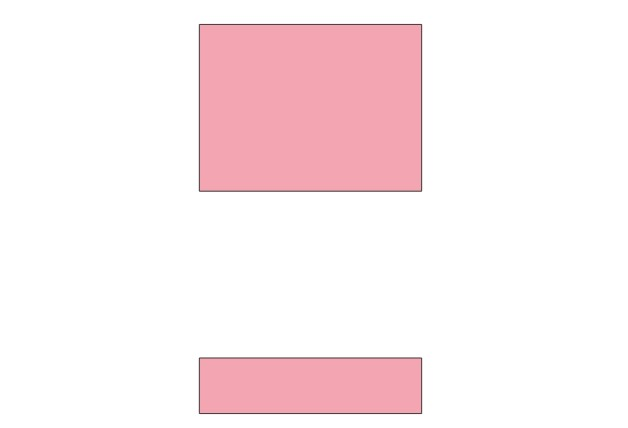
\includegraphics[width=6cm]{figures/Tugas2/1174087/no9.jpg}
		\centering
		\caption{Polygon (Bidang)}
	\end{figure}
	\item Nomor 10
	\lstinputlisting{src/tugas2/1174087/no10.py}
	\begin{figure}[H]
		
\includegraphics[width=6cm]{figures/Tugas2/1174087/no10.jpg}
		\centering
		\caption{Polygon, Hasil modulus dari npm saya 1174087 adalah 7 jadi membuat bidang segitiga siku-siku dan angka kedua dari belakang dari npm saya adalah 8 jadi membuat bidangnya sebanyak 8}
	\end{figure}
\end{enumerate}
\subsection{Link}
https://youtu.be/H9OH07pNo18